\chapter{Regression}
Regression is a very important topic in statistics that is applied extremely
frequently. There are many different kinds of regression, but in 331 we will
mostly focus on linear regression. This gives us a nice familiar example
example to demonstrate how Bayesian statistics works and how it is different
from classical or frequentist statistics. Here we will study an example of a
simple linear regression problem taken from STATS 201.

\section{A Simple Linear Regression Problem}
Data were collected from random sample of 30 drivers. The age of the driver and the 
maximum distance at which they could read a newly designed road sign were 
recorded. It is of interest to build a simple model that can be used to predict the 
maximum distance at which the sign is legible, using the age of the driver. The file 
{\tt road.txt} contains the data. Figure~\ref{fig:road} is a plot of the data:
\begin{figure}
\begin{center}
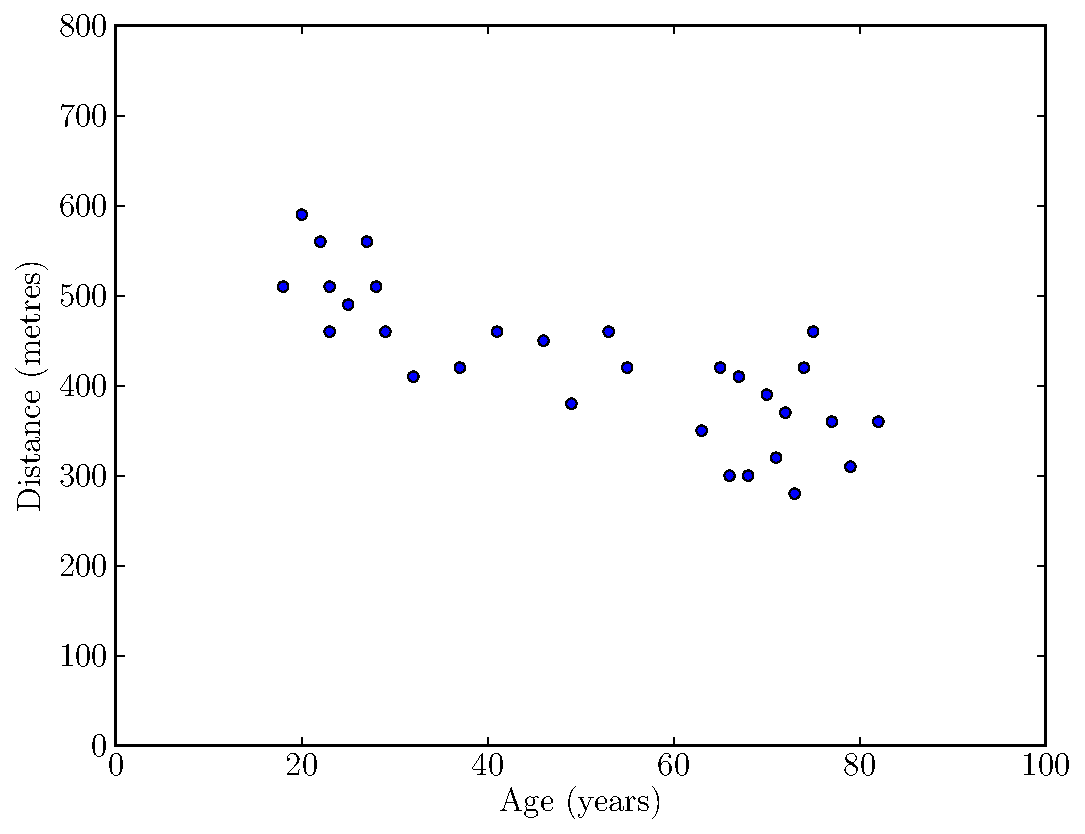
\includegraphics[scale=0.5]{Figures/road.pdf}
\caption{The distance at which a person can read a road sign, vs. the age of
the person. There are $N=30$ data points. You can clearly see that older people
have, on average, worse eyesight. But let's do a Bayesian analysis!\label{fig:road}}
\end{center}
\end{figure}
The purpose of simple linear regression is to find a straight line that goes
throught the data points. The slope and intercept of the straight line are then
helpful for understanding what is going on. Also, the straight line can be used
to predict future data, such as the maximum distance for reading the sign for a
person who is 100 years old. The most common method for obtaining the straight
line is to find the line (i.e. the slope and intercept values) that fits best
by the criterion of ``least squares''.

\section{Interpretation as a Bayesian Question}
From what you now know about Bayesian statistics, you might be able to come up
with some thoughts for what is unsatisfactory about the standard least squares
solution to linear regression. One glaring issue is that the data are {\it never
good enough} to tell us with certainty that a particular slope and intercept
are correct. In principle, we will always have uncertainty about the slope and
the intercept. From a Bayesian perspective, instead of trying to find a single
guess for the value of the slope and intercept, we should calculate the
{\it posterior distribution for the slope and the intercept, given the data}.
The posterior distribution will tell us exactly how much uncertainty we have,
and we will be able to make summaries such as point estimates and credible
intervals from that.

The equation for a straight line is usually written as $y = mx + b$ where $m$
is the gradient/slope and $b$ is the intercept.. However,
for consistency with later, more complex regression models, we will write the
equation as:
\begin{eqnarray}
y = \beta_0 + \beta_1 x.
\end{eqnarray}
Here, $\beta_0$ is the $y$-intercept and $\beta_1$ is the slope. Our goal is
to calculate the posterior distribution for $\beta_0$ and $\beta_1$ given the
data.

\section{Analytical Solution With Known Variance}
Bayes' rule (parameter estimation version) tells us how to calculate the
posterior distribution:
\begin{eqnarray}
p(\boldsymbol{\theta}|\boldsymbol{D}) \propto p(\boldsymbol{\theta})p(\boldsymbol{D}|\boldsymbol{\theta})
\end{eqnarray}
This is the general form for parameters $\boldsymbol{\theta}$ and data
$\boldsymbol{D}$. In our particular case, the
unknown parameters are $\beta_0$ and $\beta_1$, and the data are the
$y$ values of the data points. The data also consist of a number $N$ of points,
and the $x$-values,
but we shall assume that these on their own provide no information about the
slope and intercept (it would be a bit strange if they did). So the $x$-values
and the number of points $N$ act like prior information that lurks ``in the
background'' of this entire analysis.

Therefore, Bayes' rule {\it for this problem} (i.e. with the actual names
of our parameters and data, rather than generic names) reads:
\begin{eqnarray}
p(\beta_0, \beta_1 | y_1, y_2, ..., y_N) \propto
p(\beta_0, \beta_1)p(y_1, y_2, ..., y_N | \beta_0, \beta_1)
\end{eqnarray}

Let's assume uniform priors for both $\beta_0$ and $\beta_1$, and that the
prior for these two parameters are independent. The probability density for
a uniform prior distribution can be written simply as:
\begin{eqnarray}
p(\beta_0, \beta_1) \propto 1.
\end{eqnarray}
Note that we have written proportional instead of equals. If we decided to
place the limits at -1000 and 1000 (say) then the actual value of the density
would be $10^{-6}$. But this is just a number and in the end, when we normalise
the posterior distribution it won't matter. So we can just act as though the
density is proportional to 1: that is, it is a constant density, the density
is the same no matter where you go in the set of possible $\beta_0$ and $\beta_1$
values.

Now, on to the likelihood. There are $N$ data points and so there are $N$
$y$-values in the dataset, called $\{y_1, y_2, ..., y_N\}$. If we
knew the true values of $\beta_0$ and $\beta_1$, then we would predict the
$y$-values to be scattered around the straight line, with the probability
distribution for the amount of scatter given by a normal distribution with
standard deviation $\sigma$ (that we shall assume is known for the time being),
and the amount of scatter is independent for
each data point. In statisticians' notation, this can be written as:
\begin{eqnarray}
y_i \sim \mathcal{N}(\beta_0 + \beta_1 x_i, \sigma^2).
\end{eqnarray}
It is implied that all of the data values are independent (if we knew the
parameters). Therefore the likelihood can be written as a product of $N$
normal densities, one for each data point:
\begin{eqnarray}
p(\{y_1, y_2, ..., y_N\}|\beta_0, \beta_1) &=& \prod_{i=1}^N \frac{1}{\sigma\sqrt{2\pi}}
\exp\left[-\frac{1}{2\sigma^2}\left(y_i - (\beta_0 + \beta_1 x_i)\right)^2\right].
\end{eqnarray}
Remember that when we combine the likelihood with the prior using Bayes' rule,
we can usually ignore any constant factors out the front that do not depend on
the parameters. This allows us to ignore the first part of the product, outside
the exponential.
\begin{eqnarray}
p(\beta_0, \beta_1 | y_1, y_2, ..., y_N) &\propto& p(\beta_0, \beta_1)
p(y_1, y_2, ..., y_N|\beta_0, \beta_1)\\
&\propto& 1 \times \prod_{i=1}^N \exp\left[-\frac{1}{2\sigma^2}\left(y_i - (\beta_0 + \beta_1 x_i)\right)^2\right]\\
&\propto& \exp\left[-\frac{1}{2\sigma^2}\sum_{i=1}^N\left(y_i - (\beta_0 + \beta_1 x_i)\right)^2\right].
\label{eq:leastsquares}
\end{eqnarray}
This is the posterior distribution! Note that it is hard to interpret just by
looking at it, but it
is in fact what we need, because for any possible values of $\beta_0$ and $\beta_1$
we could evaluate this equation and work out the posterior probability density.

There are a few things you should note about the posterior distribution in
Equation~\ref{eq:leastsquares}. Firstly, the way it depends on the parameters
is that it is an exponential of something involving the parameters $\beta_0$
and $\beta_1$ in linear and second-order ways (if you were to expand the square,
you would get terms like $\beta_0\beta_1$ and $\beta_0^2$). Mathematicians would
say that the thing inside the exponential sign is a quadratic form. When a
probability density can be written as the exponential of a quadratic form, it
is a normal density. Therefore the posterior distribution for $\beta_0$ and
$\beta_1$ is a (bivariate) normal distribution in this case.

Secondly, take another look at the sum term. Do you recognise it, or can you
figure out what it means? The sum term is nothing more than the sum of squared
residuals between the data and the straight line implied by the parameters!
In standard least squares linear regression, $\beta_0$ and $\beta_1$ are
estimated by minimising this sum of squared residuals. Because of the exp and
the minus sign, what the posterior distribution tells us is that the choice of
$\beta_0$ and $\beta_1$ that minimises the sum of squared residuals, maximises
the posterior probability density.

\begin{framed}
\begin{center}
{\bf Doing a linear regression by least squares is equivalent to having a
uniform prior and a normal likelihood, and finding the posterior mode.}
\end{center}
\end{framed}

\section{Solution With JAGS}
The above results made one major unrealistic assumption: that the standard
deviation $\sigma$, or scatter, was known. In practice, it usually needs to be
estimated from the data as well. Therefore, in the Bayesian framework, we should
have it be an unknown parameter. Now we have three unknown parameters instead
of two: these are the intercept of the straight line, the gradient of
the straight line, and the standard deviation of the noise or scatter.
\begin{eqnarray}
\boldsymbol{\theta} = \{\beta_0, \beta_1, \sigma\}.
\end{eqnarray}
One major advantage of MCMC is that we can increase the number of unknown parameters
without having to worry about the fact that the posterior distribution might
be hard to interpret or plot.

The data is the same as before:
\begin{eqnarray}
\boldsymbol{D} = \{y_1, y_2, ..., y_N\}
\end{eqnarray}
and so is the likelihood:
\begin{eqnarray}
y_i \sim \mathcal{N}(\beta_0 + \beta_1 x_i, \sigma^2).
\end{eqnarray}

Our three parameters will need priors. JAGS requires proper priors (i.e. we
can't have a uniform prior over an infinite range), so we will have to be a
little careful about that. Instead of using uniform distributions this time,
we will use normal distributions with a mean of 0 and a large standard deviation
of 1000.

For the standard deviation parameter $\sigma$, we know firstly that this cannot
be negative. Let's use a log-uniform prior with generous lower and upper limits,
so we express uncertainty about the order of magnitude of $\sigma$.
In JAGS, the model looks like this:
\begin{framed}
\begin{verbatim}
model
{
    # Prior for all the parameters
    beta0 ~ dnorm(0, pow(1E3, -2))
    beta1 ~ dnorm(0, pow(1E3, -2))
    log_sigma ~ dunif(-10, 10)
    sigma <- exp(log_sigma)

    # Likelihood
    for(i in 1:N)
    {
        y[i] ~ dnorm(beta0 + beta1*x[i], pow(sigma, -2))
    }
}
\end{verbatim}
\end{framed}
The first part defines the priors for the parameters. For $\beta_0$ and $\beta_1$,
we have just chosen very broad priors that describe vague prior knowledge. Note
that the standard deviations of the priors are 1000, so we should be careful
to only apply this code to situtations where we don't expect the intercept or
slope to take on an extreme value.

For the standard deviation parameter $\sigma$ which describes how much we
expect the data points to be scattered around the straight line, we have assigned
a log-uniform prior. The limits of $-10$ and $10$ for {\tt log\_sigma} imply
limits of $4.5 \times 10^{-5}$ to 22,000 for {\tt sigma}, a generous range.
Again, if we thought the scatter
was going to be outside this range, we should change the prior to something
else or risk getting strange answers.

\chapter{Simple Linear Regression With Outliers}
One complication that is common in linear regression (or other model-fitting)
problems is the existence of outliers. These are points that do not fit in with
the general trend. If these are left in the analysis, the results can easily
be incorrect. Many methods exist for deciding how to ``detect'' and ``remove''
outliers. In lectures and labs we will study and extension to the simple linear
regression model that allows for outliers. Rather than simply ``rejecting'' some
points as outliers, we can leave them in, but there will be a posterior probability
that each point is an outlier! That way, all points can contribute to the results.
Information is not wasted.



